\documentclass[12pt]{article}

\usepackage{times}
\usepackage{graphicx}
\usepackage{datetime}
\usepackage[utf8]{inputenc}
\usepackage[slovene]{babel}
\usepackage[font=]{caption}

\usepackage{listings}
\usepackage{color}
\usepackage{dirtree}

\definecolor{folderbg}{RGB}{124,166,198}
\definecolor{folderborder}{RGB}{110,144,169}

\definecolor{dkgreen}{rgb}{0,0.6,0}
\definecolor{gray}{rgb}{0.5,0.5,0.5}
\definecolor{mauve}{rgb}{0.58,0,0.82}
\definecolor{darkblue}{rgb}{0.0,0.0,0.6}

\lstset{
	basicstyle=\ttfamily,
	columns=fullflexible,
	showstringspaces=false,
	commentstyle=\color{gray}\upshape
}

\lstdefinelanguage{XML}
{
	morestring=[b]",
	morestring=[s]{>}{<},
	morecomment=[s]{<?}{?>},
	stringstyle=\color{black},
	identifierstyle=\color{darkblue},
	keywordstyle=\color{cyan},
	morekeywords={xmlns,version,type}
}

\lstdefinestyle{XmlStyle}{
	language=XML,
	aboveskip=3mm,
	belowskip=3mm,
	showstringspaces=false,
	columns=flexible,
	basicstyle={\small\ttfamily},
	numbers=none,
	keywordstyle=\color{blue},
	breaklines=true,
	tabsize=4
}

\lstdefinestyle{JavaStyle}{
	language=Java,
	aboveskip=3mm,
	belowskip=3mm,
	showstringspaces=false,
	columns=flexible,
	basicstyle={\small\ttfamily},
	numbers=none,
	numberstyle=\tiny\color{gray},
	keywordstyle=\color{blue},
	commentstyle=\color{dkgreen},
	stringstyle=\color{mauve},
	breaklines=true,
	tabsize=4
}

\newdateformat{MMYYYYdate}{\monthname[\THEMONTH] \THEYEAR}
\title{RIPtide - Univerzalno orodje za konfiguracijo omrežij}
\author{Jurij Fortuna, G 3. a}
\date{\MMYYYYdate\today}

\begin{document}

\begin{center}
	\thispagestyle{empty}
	
\includegraphics[scale=1]{slike/vegova.png}

	\vspace{\fill}
	Seminarska naloga pri predmetu računalništvo

	\Huge{RIPtide - Univerzalno orodje za konfiguracijo omrežij}

	\normalsize
	\vspace{\fill}

	Mentor: Marko Kastelic, prof. \hfill Avtor: Jurij Fortuna , G 3. a\\
	\null
	Ljubljana, \MMYYYYdate\today
\end{center}
\newpage

% Povzetek
\section*{Povzetek}
V tej seminarski nalogoje opisan razvojni proces in delovanje programa
RIPtide. RIPtide je odprtokodna programska oprema, razvita v jeziku Java,
namenjena konfiguriranju omrežnih naprav. Odpravlja problem uporabe
različne programske opreme različnih proizvajalcev za konfiguriranje
omrežne opreme. Na začetku dokumenta je podan kratek pregled dveh glavnih
komponent programske opreme: uporabniškega vmesnika (frontend) in
programskega vmesnika aplikacij (API). V nadaljevanju dokument opisuje
''Shede'', vtičnike za interakcijo z omrežno opremo. Članek se zaključi z
opisom razvoja Sheda in obravnava izzive, povezane z njim.
\\\\
\textbf{Ključe besede:} konfiguracija omrežij, omrežja, vtičniki, API,
odprtokodna programska oprema
\\
\section*{Abstract}
\foreignlanguage{english}{
	The purpose of this paper is to report on the development process and
	inner workings of RIPtide. RIPtide is an open-source software developed
	in Java for configuring network devices. It addresses the issue of
	using multiple software solutions from different manufacturers to
	configure networks. Initially, the document gives a brief overview of
	two main components of the software: the frontend and the Application
	Programming Interface (API). Following that, the document describes
	''Sheds,'' plugins for interacting with network equipment. The paper
	concludes by documenting the development of a custom Shed and discusses
	the associated challenges that can arise during the development.
	\\\\
	\textbf{Keywords:} network configuration, networking, plugins, API,
	open-source software
}
\newpage

% Kazalo
\tableofcontents
\newpage

% 1. Uvod
\section{Uvod}
Ideja za razvoj RIPtide-a se je pojavila, ko sem bil med konfiguracijo
domačega omrežja prisiljen uporabljati tri različne programske opreme,
različnih proizvajalcev. Med sabo so se nemalo razlikovale in so bile
po večini nestabilne. Zato sem se odločil razviti generično programsko
opremo za konfiguracijo omrežij. Deluje na principu
“vtičnikov” (t.i. Shedov) za posamezne kose omrežne opreme.\\\\\\

\begin{center}
	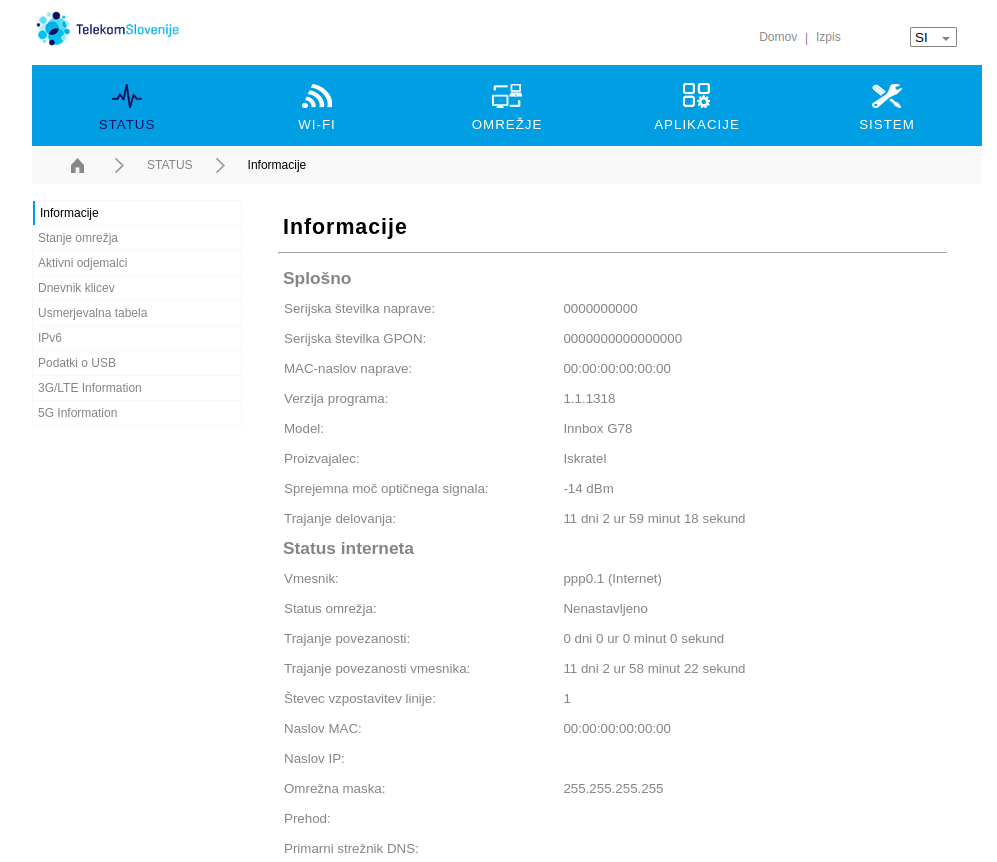
\includegraphics[scale=0.5]{slike/telekom.png}
	\captionof{figure}{Primer konfiguracijske strani za usmerjevalnike Telekoma Slovenije}
\end{center}
\newpage

% 2. Tehnologije
\section{Uporabljene tehnologije}
Tako Shedi, kot tudi RIPtide so napisani v Javi. Java omogoča dinamično
nalaganje modulov ob zagonu navideznega stroja, tudi iz zapakiranih JAR
datotek. Sam RIPtide je zgrajen iz dveh glavnih delov: osprednega dela 
in aplikacijskega programskega vmesnika (v nadaljevanju API).
Poleg tega velja omeniti Shede, ki jih lahko razvije kdorkoli z uporabo
RIPtide API-ja.
\newpage

% 3. Ospredni del
\section{Ospredni del}
Ospredni del je odgovoren za konfiguracijo RIPtide-a ter rokovanje z 
uporabnikovimi poverilnicami in napravami.

\subsection{Konfiguracija}
Uporabnik lahko svoje naprave shrani, in si s tem prihrani čas za
morebitno kasnejšo konfiguracijo. Poleg tega RIPtide omogoča spremembo
barve vmesnika po uporabnikovi želji.

\subsubsection{Shranjevanje podatkov}
Okoljske spremenljivke, naprave in poverilnice so zapisanje v objektu
imenovanem \texttt{Workspace}.

\begin{lstlisting}[style=JavaStyle]
@Data
public class Workspace implements Serializable {
	private Theme theme;
	private ArrayList<Credential> credentials;
	private ArrayList<Connection> connections;

	public Workspace() {
		theme = Theme.PRIMER_DARK;
		credentials = new ArrayList<>();
		connections = new ArrayList<>();
	}

	public Workspace(Theme theme, ArrayList<Credential> credentials, ArrayList<Connection> connections) {
		this.theme = theme;
		this.credentials = credentials;
		this.connections = connections;
	}
}
\end{lstlisting}
Ko uporabnik nastavitve shrani je objekt serializiran in zapisan v datoteko
na uproabnikov sistem. Datotek je lahko več, kar omogoča prilagoditev
vmesnika za različna okolja (npr. posebej za domačo in poslovno rabo).
Workspace datoteke so shranjene v JSON formatu, kar uporabnikom omogoča
enostavno izmenjavo ali prenos.

\subsubsection{Barve vmesnika}
Uporabnik lahko vmesnik prilagodi na štiri priložene teme. V prihodnosti
bo mogoče nalaganje barv iz CSS datoteke po meri.

\subsection{Upravljanje poverilnic}
Za konfiguracijo večine omrežnih naprav je potrebna avtorizacija.
RIPtide uporabnikom omogoča varno shranjevanje poverilnic na njihovem
sistemskem keyringu. Poverilnice so ob povezavi na napravo prek API-ja
podani Shedu, kar pomeni, da se razvijalci teh ne rabijo ukvarjati z
varnim hranjenjem poverilnic.

\subsection{Rokovanje z napravami}
\subsubsection{Nalaganje Shedov}
Nalaganje shedov poteka v dveh korakih, lociranje Sheda in branje
metapodatkov. Na uporabnikovem sistemu se nahajajo v obliki JAR datotek v
dveh mapah, \texttt{\textasciitilde/.config/RIPtide/sheds} na NIX sistemih
in \texttt{\%UserProfile\%\textbackslash\\.RIPtide\textbackslash sheds} na
Windows sistemih.

\subsubsection{Nalaganje naprav} \label{nalaganje-naprav}
Ob izbiri naprave, RIPtide iz Shedovih metapodatkov najprej prebere
njen t.i. model path, ki izgleda približno
tako: \texttt{telekomslovenije.innboxg78.ts}. Niz je sestavljen iz ID-ja
Sheda, ID-ja modela nprave in ID-ja različice modela. Vsi ID-ji so
edinstveni, kar pomeni, da lahko program najde Shed, v njem poišče model
naprave, njegovo različico in vzpostavi povezavo z napravo prek API-ja.
\newpage

% 4. Aplikacijski programski vmesnik
\section{Aplikacijski programski vmesnik}
API omogoča uporabnikom, da ustvarijo lastno podporo za omrežno
opremo, ki je programska oprema še ne podpira. To pomeni, da lahko
skrbniki omrežij enostavno integrirajo nove naprave v svoje omrežje, ne da
bi morali čakati, da prodajalec izda uradno podporo.

\subsection{Dostop do API-ja}
Dostop do APIja je mogoč preko SDK knjižnice. Nahaja se v RIPtide
Maven repozitoriju. Ker so Javanski upravitelji paketov med seboj bolj
kot ne kompatibilni, je tudi postopek dodajanja knjižnice med njimi
zelo podoben. Več o projektni strukturi pa v razdelku
\ref{projektna-struktura}.

\subsection{Struktura API-ja}
Vsi pomembni vmesniki in razredi za pisanje Shedov se nahajajo v
paketu \texttt{org\-.riptide.sdk.sheds}. Paket je deljen na podpakete za
uporabniški vmesnik, tipe naprav, čarovnike in avtentikacijo.

\subsection{Vgrajena orodja}
API vsebuje uporabna orodja za izdelovanje statusnih strani in
formularjev, ki se nahajajo v paketu \texttt{org.riptide.sdk.sheds.ui}.

\subsection{Komunikacija z napravami} \label{komunikacija-z-napravami}
Ospredni del s Shedi komunicira preko vmesnikov. Za primer vzemimo
Telekomov usmerjevalnik. Ob izbiri naprave se instancira njen gonilni
razred v nov objekt, ki je odgovoren za komunikacijo z napravo
(postopek je opisan v razdelku \ref{nalaganje-naprav}).
\\\\
Program iz metapodatkov razbere, da naprava tipa router. To pomeni,
da mora njen gonilni razred implementirati vmesnik \texttt{Router} in
posledično \texttt{Device}, saj ga \texttt{Router} razširja.
\newpage

\begin{lstlisting}[style=JavaStyle]
public interface Device {
	void initialize(String address, Credential credential);
	TreeMap<String, Tab[]> getPages();
}

public interface Router extends Device {
	PATWizard patWizard();
}
\end{lstlisting}
Za tem se kliče metoda \texttt{initialize/2}, ki gonilnemu objektu poda
omrežni naslov naprave in poverilnice.
\\\\
Nato program od gonilnega objekta zahteva seznam konfiguracijskih strani
in zavihke z metodo \texttt{getPages/1}. Strani so predstavljene s tabelami
\texttt{Tab} objektov, ki so preslikane v nize. Shedi imajo običajno razrede,
ki implementirajo vmesnik \texttt{Tab}, ti se instancirajo in vrnejo v
metodi. Ospredni del nato z orodnim razredom \texttt{ContentRenderer}
generira stran, kot je prikazana spodaj.

\begin{center}
	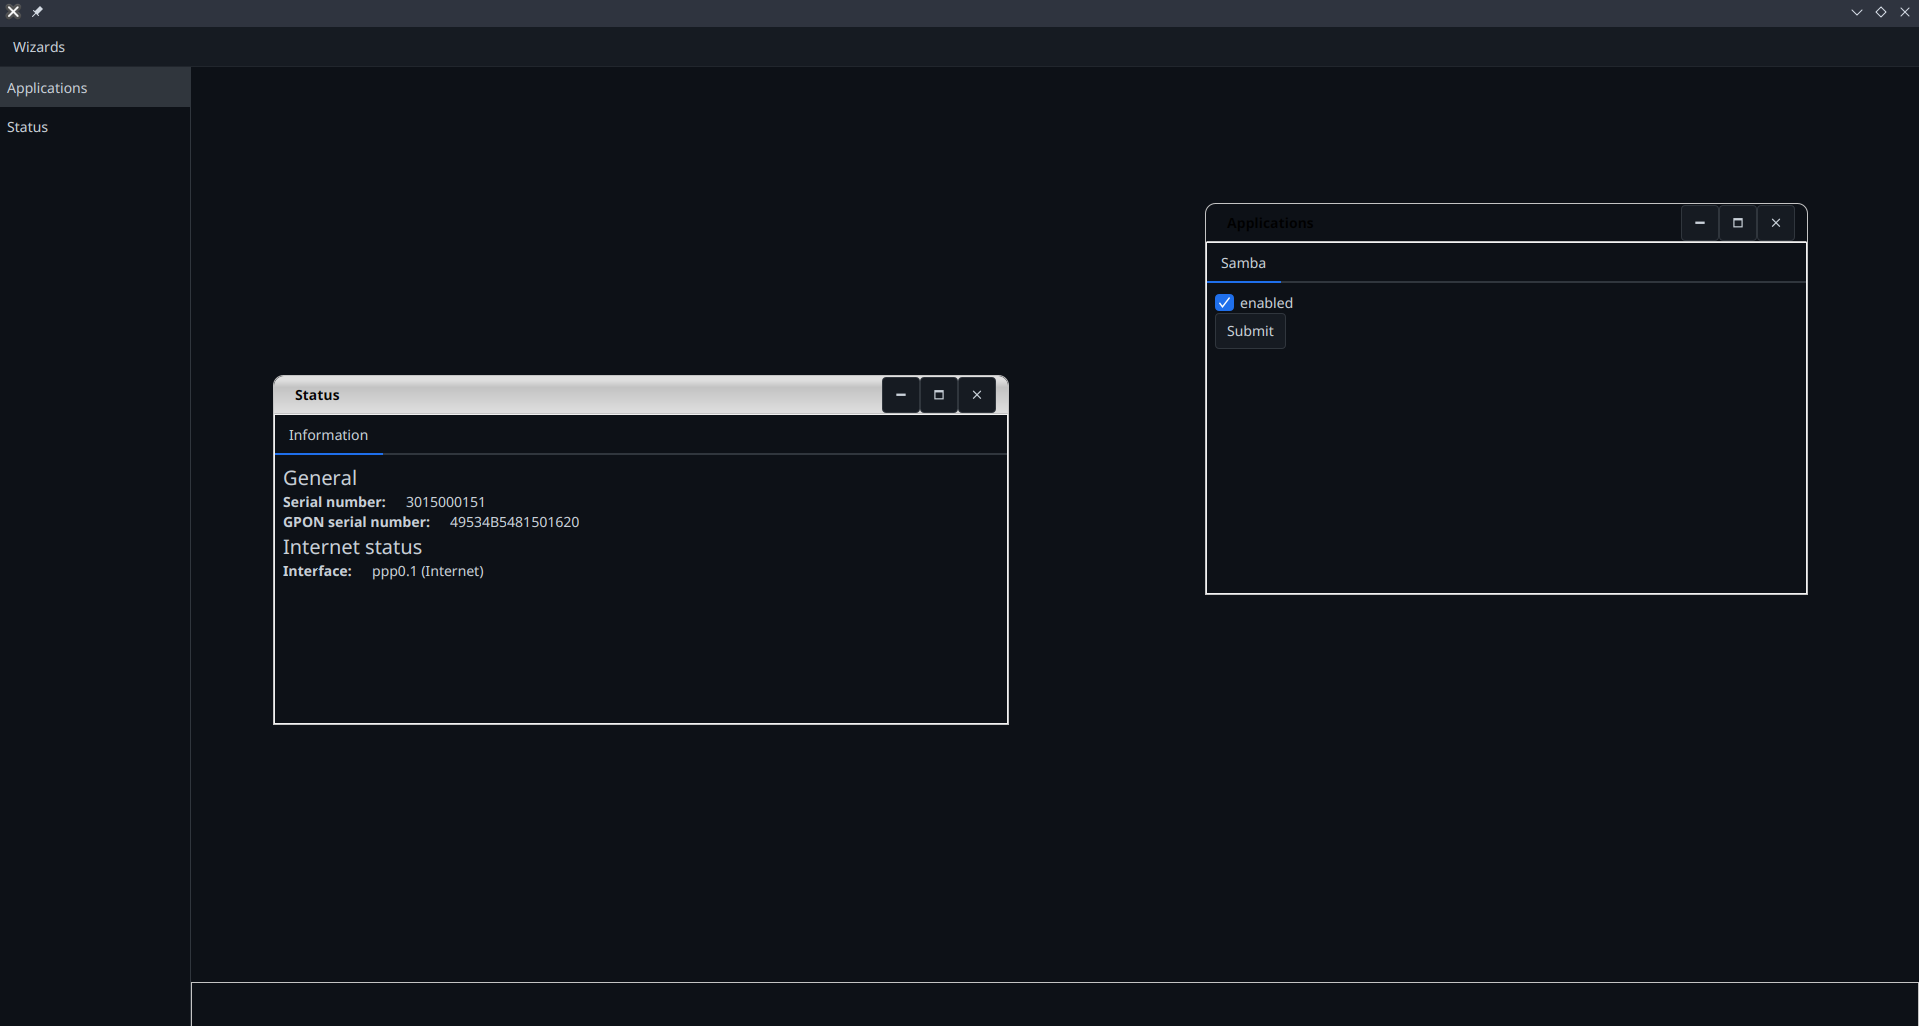
\includegraphics[scale=0.28]{slike/config-window.png}
	\captionof{figure}{Primer generirane konfiguracijske strani}
\end{center}
\newpage

\subsection{Čarovniki}
Program tudi manj naprednim uporabnikom omogoča konfiguracijo njihove
omrežne opreme. Na konfiguracijski strani za katerokoli omrežno napravo
se v menijski vrstici nahaja gumb ''Wizards''. Pod njem se glede na tip
naprave pojavijo različne podmožnosti. Za usmerjevalnike je to zaenkrat
\textit{Port forwaring wizard}, ki omogoča uporabniku konfiguracijo
preusmerjanja protokolnih vrat, za stikala pa \textit{VLAN wizard},
ki omogoča konfiguracijo shranjenih VLAN-ov.

\subsubsection{Implementacija čarovnikov}

\newpage

% 5. Shedi
\section{Shedi}
Za komunikacijo z napravami RIPtide preko API-ja uporablja Shede. Shedi
sami po sebi niso izvršljivi programi, vendar so le zbirka razredov.
Zapakirani so v JAR datoteke, skupaj z datoteko \texttt{shed.yml}.
\\\\
V prihodnosti načrtujem omogočiti razširitev tudi drugih funkcionalnosti.
Zaradi tega sem se za poimenovanje vtičnikov naprav odločil uporabiti
izraz ''shedi'' namesto običajnega izraza ''plugin''.

\subsection{Priprava projekta}
Zaradi olajšanja dela, projekt naredimo s pomočjo upravitelja paketov. V
tem poglavju bom delal s pomočjo uporavitelja \textit{Apache Maven}. Za
začetek je potrebno dodati repozitorij in knjižnico. To naredimo v datoteki
\texttt{pom.xml}.

\begin{lstlisting}[style=XmlStyle]
<repositories>
	<repository>
		<id>repsy</id>
		<url>https://repo.repsy.io/mvn/riptide/maven</url>
	</repository>
</repositories>

<dependencies>
	<dependency>
		<groupId>org.riptide</groupId>
		<artifactId>sdk</artifactId>
		<version>VERZIJA</version>
	</dependency>
</dependencies>
\end{lstlisting}
\newpage

\subsection{Projektna struktura} \label{projektna-struktura}
\begin{dirtree}{%
.1 NasShed.
	.2 src.
		.3 main.
			.4 java.
				.5 organizacija.
					.6 artefakt.
						.7 GonilniRazred.java.
			.4 resources.
				.5 shed.xml.
	.2 pom.xml.
}
\end{dirtree}
\vspace*{12pt}
V privzeti paket (oziroma podpakete) dodamo gonilne razrede za naše naprave.
V \texttt{resources} mapo pa datoteko \texttt{shed.yml}, ki bo vsebovala
metapodatke o Shedu.

\subsubsection{Metapodatki}
Metapodatki vsebujejo pomembne podatke o Shedu, ki so nujni za delovanje.

\begin{lstlisting}[style=XmlStyle]
name: "Telekom Slovenije Shed"
id: "telekomslovenije"
version: "1.0"
api_level: "1.0"
authors:
	- "chocoearly44"
routers:
	- name: "InnboxG78"
	id: "innboxg78"
	flavours:
		- name: "Telekom Slovenije"
		id: "ts"
		handler: "org.riptide.ts.Main"
switches:
\end{lstlisting}
Zaglavje vsebuje ime Sheda, njegov ID, verzijo, avtorje in podprto verzijo
API-ja, za katero je bil zgrajen. Pod zaglavjem sledijo razdelki s tipi
naprav. V njih so shranjene podprte naprave, ki vsebujejo imena, ID-je in
vrste. Vrste vsebujejo gonilne razrede, saj ima naprava lahko različne
funkcionalnosti, glede na nameščeno programsko opremo. Tako zagotovimo
da lahko Shed podpira isto napravo, ne glede na distributorja (za primer
InnboxG78 usmerjevalnik, ki ga distribuirata tako Telekom Slovenije, kot
tudi T2).

\subsubsection{Gonilni razredi}


\subsubsection{Zavihki}
\subsection{Izgradnja in uporaba}
\newpage

% 6. Eksperimentalne funkcije
\section{Eksperimentalne funkcije}
RIPtide je opremljen z nekaj novimi eksperimentalnimi funkcijami,
ki pa jih zaradi pomanjkanja časa nisem uspel povsem dokončati in
stestirati. Te omogočajo naprednim uporabnikom nove možnosti avtomacije
in pregleda nad omrežjem.

\subsection{Topološki pogled omrežja}
\newpage

% 7. Zaključek
\section{Zaključek}
\newpage

\end{document}